\chapter{Graph Neural Networks}
% Authors: Yu Cao 5/7/19.

\section{Graph Neural Network}
Graph contains vertexes and edges and the messages(information) associated, and can be used to formalize Images and texts. Deep learning on graph structure composes GNN. GNN learns embedding on graphs. 

\begin{figure}[ht]
\begin{center}
% \fbox{\rule{0pt}{2in} \rule{0.9\linewidth}{0pt}}
%   \includegraphics[width=0.9\linewidth]{imgs/PnL_Problem}
  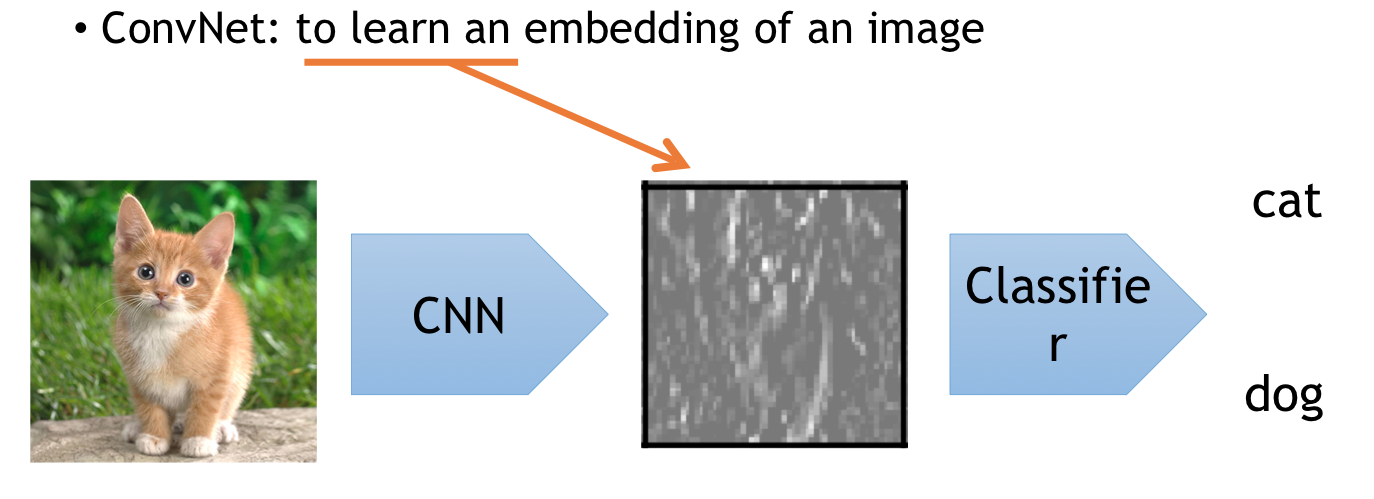
\includegraphics[width=3.38in]{figs/Embedding_ConvNet.png}
\end{center}
   \caption{ConvNets: Learn embedding of an image}
\label{fig:CV}
\end{figure}

\begin{figure}[ht]
\begin{center}
% \fbox{\rule{0pt}{2in} \rule{0.9\linewidth}{0pt}}
%   \includegraphics[width=0.9\linewidth]{imgs/PnL_Problem}
  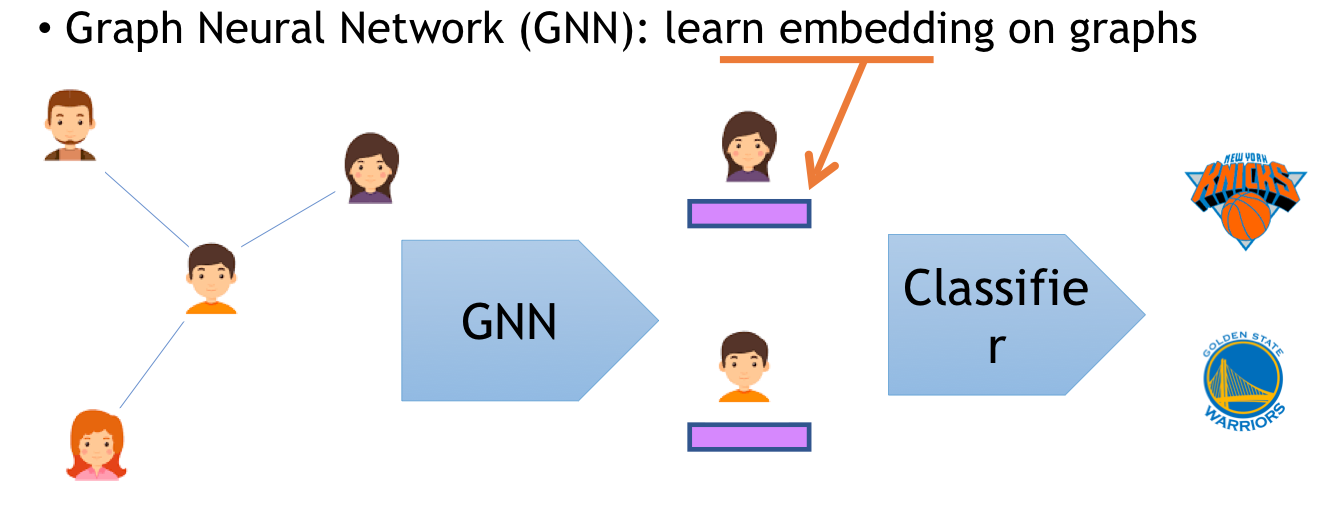
\includegraphics[width=3.38in]{figs/Embedding_Graph.png}
\end{center}
   \caption{Graph Neural Network: Learn embedding on graphs}
\label{fig:CV}
\end{figure}

It is widely applied in the tasks of Natural Language Processing. Medical Computation as well as Computer Vision as shown on figures 3, 4 and 5 below.. 
\begin{figure}[ht]
\begin{center}
% \fbox{\rule{0pt}{2in} \rule{0.9\linewidth}{0pt}}
%   \includegraphics[width=0.9\linewidth]{imgs/PnL_Problem}
  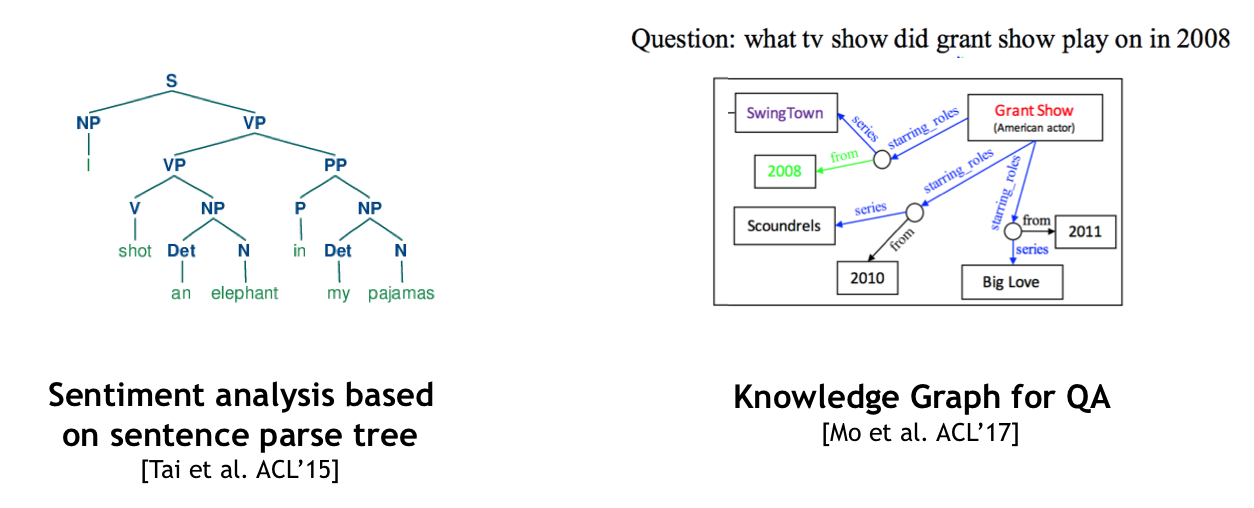
\includegraphics[width=3.38in]{figs/NLP.png}
\end{center}
   \caption{Application in NLP}
\label{fig:CV}
\end{figure}

\begin{figure}[ht]
\begin{center}
% \fbox{\rule{0pt}{2in} \rule{0.9\linewidth}{0pt}}
%   \includegraphics[width=0.9\linewidth]{imgs/PnL_Problem}
  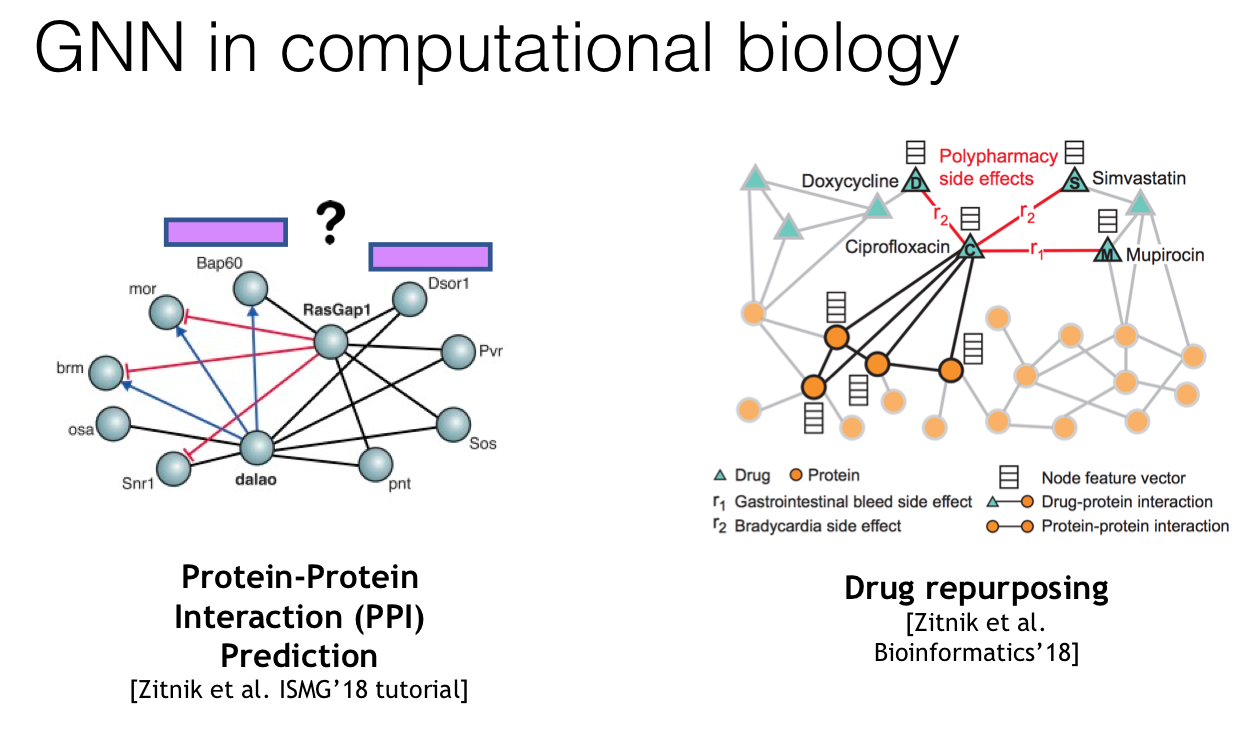
\includegraphics[width=3.38in]{figs/Biology.png}
\end{center}
   \caption{Application in Biology}
\label{fig:CV}
\end{figure}

\begin{figure}[ht]
\begin{center}
% \fbox{\rule{0pt}{2in} \rule{0.9\linewidth}{0pt}}
%   \includegraphics[width=0.9\linewidth]{imgs/PnL_Problem}
  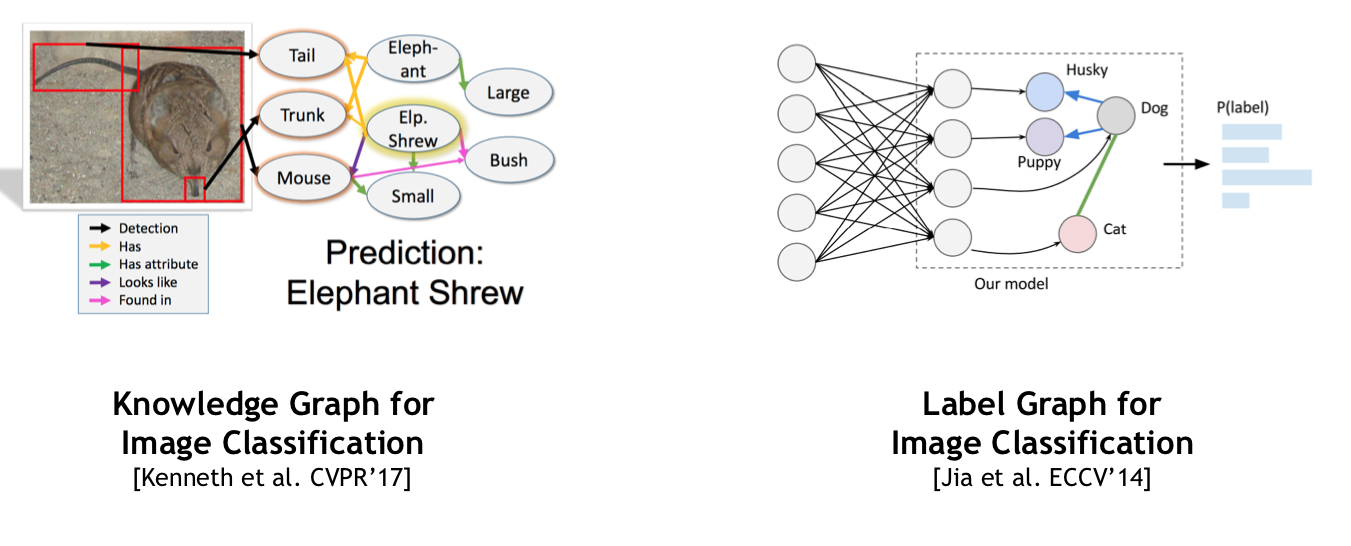
\includegraphics[width=3.38in]{figs/Computer_Vision.png}
\end{center}
   \caption{Application in Computer Vision}
\label{fig:CV}
\end{figure}


Graph neural network has been an emerging topic of research as shown in the graph below

\begin{figure}[ht]
\begin{center}
% \fbox{\rule{0pt}{2in} \rule{0.9\linewidth}{0pt}}
%   \includegraphics[width=0.9\linewidth]{imgs/PnL_Problem}
  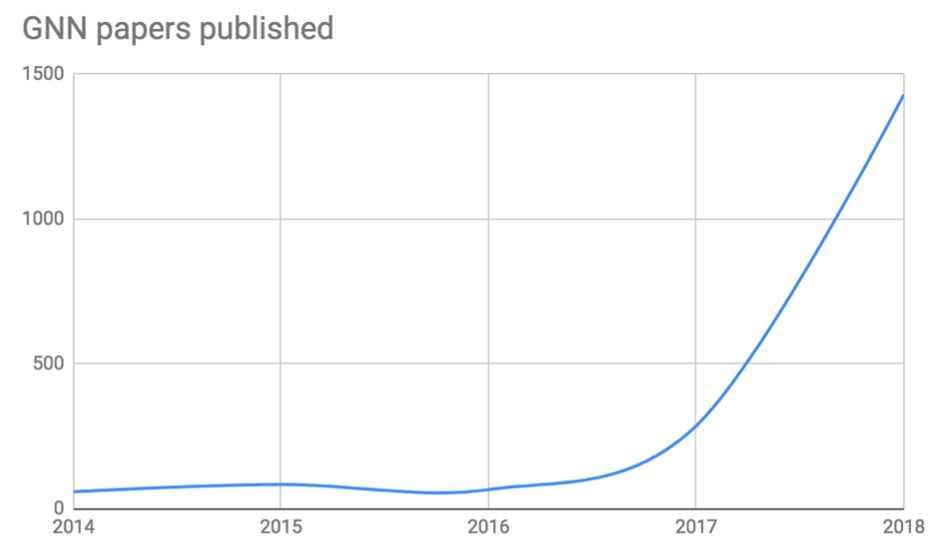
\includegraphics[width=3.38in]{figs/GNN Papers Published.png}
\end{center}
   \caption{GNN papers published}
\label{fig:CV}
\end{figure}

\section{Message passing on graph}
 In this section, we will focus on how to perform computation on graph structures following Message Passing paradigm. Many graph neural networks follows the \textit{message passing} computation model \href{https://arxiv.org/abs/1704.01212}{Gilmer et al, 2017}:
\begin{itemize}
    \item Each node receives and aggregates messages from its neighbors  
\begin{gather}
m_v^{t+1} = \sum\limits_{w\in \mathcal{N}(v)}M_t(h_v^t, h_w^t, e_{vw}^t)
\end{gather}
where $\mathcal{N}(v)$ is the neighbour set of node $v$.

\item Each node update its own embedding using aggregated messages.
\end{itemize}
% [(a)]
% \item
% Each node receives and aggregates messages from its neighbors  
% % \begin{gather}
% $$m_v^{t+1} = \sum\limits_{w\in \mathcal{N}(v)}M_t(h_v^t, h_w^t, e_{vw}^t)$$
% % \end{gather}
% where $\mathcal{N}(v)$ is the neighbor set of node $v$.

% \item
% Each node update its own embedding using aggregated messages
% $$h_v^{t+1} = U_t(h_v^t, m_v^{t+1})$$

% \end{enumerate}


\section{Graph Convolutional Network}

Graph convolutional network (GCN) is a popular model proposed by \href{https://arxiv.org/abs/1609.02907}{Kipf \& Welling} to encode graph structure by message passing. The high-level idea is similar to our toy task: node features are updated by aggregating the messages from the neighbors. Here is its message passing equation:

$$
h_{v_i}^{(l+1)} = \sigma \left(\sum_{j\in\mathcal{N}(i)}\frac{1}{c_{ij}}h_{v_j}^{(l)}W^{(l)} \right),
$$

where $v_i$ is any node in the graph; $h_{v_i}$ is the feature of node $v_i$; $\mathcal{N}(i)$ denotes the neighborhood of $v_i$; $c_{ij}$ is the normalization constant related to node degrees; $W$ is the parameter and $\sigma$ is a non-linear activation function.




